
%% bare_conf.tex
%% V1.3
%% 2007/01/11
%% by Michael Shell
%% See:
%% http://www.michaelshell.org/
%% for current contact information.
%%
%% This is a skeleton file demonstrating the use of IEEEtran.cls
%% (requires IEEEtran.cls version 1.7 or later) with an IEEE conference paper.
%%
%% Support sites:
%% http://www.michaelshell.org/tex/ieeetran/
%% http://www.ctan.org/tex-archive/macros/latex/contrib/IEEEtran/
%% and
%% http://www.ieee.org/

%%*************************************************************************
%% Legal Notice:
%% This code is offered as-is without any warranty either expressed or
%% implied; without even the implied warranty of MERCHANTABILITY or
%% FITNESS FOR A PARTICULAR PURPOSE! 
%% User assumes all risk.
%% In no event shall IEEE or any contributor to this code be liable for
%% any damages or losses, including, but not limited to, incidental,
%% consequential, or any other damages, resulting from the use or misuse
%% of any information contained here.
%%
%% All comments are the opinions of their respective authors and are not
%% necessarily endorsed by the IEEE.
%%
%% This work is distributed under the LaTeX Project Public License (LPPL)
%% ( http://www.latex-project.org/ ) version 1.3, and may be freely used,
%% distributed and modified. A copy of the LPPL, version 1.3, is included
%% in the base LaTeX documentation of all distributions of LaTeX released
%% 2003/12/01 or later.
%% Retain all contribution notices and credits.
%% ** Modified files should be clearly indicated as such, including  **
%% ** renaming them and changing author support contact information. **
%%
%% File list of work: IEEEtran.cls, IEEEtran_HOWTO.pdf, bare_adv.tex,
%%                    bare_conf.tex, bare_jrnl.tex, bare_jrnl_compsoc.tex
%%*************************************************************************

% *** Authors should verify (and, if needed, correct) their LaTeX system  ***
% *** with the testflow diagnostic prior to trusting their LaTeX platform ***
% *** with production work. IEEE's font choices can trigger bugs that do  ***
% *** not appear when using other class files.                            ***
% The testflow support page is at:
% http://www.michaelshell.org/tex/testflow/



% Note that the a4paper option is mainly intended so that authors in
% countries using A4 can easily print to A4 and see how their papers will
% look in print - the typesetting of the document will not typically be
% affected with changes in paper size (but the bottom and side margins will).
% Use the testflow package mentioned above to verify correct handling of
% both paper sizes by the user's LaTeX system.
%
% Also note that the "draftcls" or "draftclsnofoot", not "draft", option
% should be used if it is desired that the figures are to be displayed in
% draft mode.
%
\documentclass[conference]{IEEEtran}
\usepackage{blindtext, graphicx}
\usepackage{hyperref}
\usepackage{caption}
\hypersetup{
    colorlinks=true,
    linkcolor=blue,
    filecolor=blue,      
    urlcolor=blue,
    citecolor   = blue
}
% Add the compsoc option for Computer Society conferences.
%
% If IEEEtran.cls has not been installed into the LaTeX system files,
% manually specify the path to it like:
% \documentclass[conference]{../sty/IEEEtran}





% Some very useful LaTeX packages include:
% (uncomment the ones you want to load)


% *** MISC UTILITY PACKAGES ***
%
%\usepackage{ifpdf}
% Heiko Oberdiek's ifpdf.sty is very useful if you need conditional
% compilation based on whether the output is pdf or dvi.
% usage:
% \ifpdf
%   % pdf code
% \else
%   % dvi code
% \fi
% The latest version of ifpdf.sty can be obtained from:
% http://www.ctan.org/tex-archive/macros/latex/contrib/oberdiek/
% Also, note that IEEEtran.cls V1.7 and later provides a builtin
% \ifCLASSINFOpdf conditional that works the same way.
% When switching from latex to pdflatex and vice-versa, the compiler may
% have to be run twice to clear warning/error messages.






% *** CITATION PACKAGES ***
%
%\usepackage{cite}
% cite.sty was written by Donald Arseneau
% V1.6 and later of IEEEtran pre-defines the format of the cite.sty package
% \cite{} output to follow that of IEEE. Loading the cite package will
% result in citation numbers being automatically sorted and properly
% "compressed/ranged". e.g., [1], [9], [2], [7], [5], [6] without using
% cite.sty will become [1], [2], [5]--[7], [9] using cite.sty. cite.sty's
% \cite will automatically add leading space, if needed. Use cite.sty's
% noadjust option (cite.sty V3.8 and later) if you want to turn this off.
% cite.sty is already installed on most LaTeX systems. Be sure and use
% version 4.0 (2003-05-27) and later if using hyperref.sty. cite.sty does
% not currently provide for hyperlinked citations.
% The latest version can be obtained at:
% http://www.ctan.org/tex-archive/macros/latex/contrib/cite/
% The documentation is contained in the cite.sty file itself.






% *** GRAPHICS RELATED PACKAGES ***
%
\ifCLASSINFOpdf
  % \usepackage[pdftex]{graphicx}
  % declare the path(s) where your graphic files are
  % \graphicspath{{../pdf/}{../jpeg/}}
  % and their extensions so you won't have to specify these with
  % every instance of \includegraphics
  % \DeclareGraphicsExtensions{.pdf,.jpeg,.png}
\else
  % or other class option (dvipsone, dvipdf, if not using dvips). graphicx
  % will default to the driver specified in the system graphics.cfg if no
  % driver is specified.
  % \usepackage[dvips]{graphicx}
  % declare the path(s) where your graphic files are
  % \graphicspath{{../eps/}}
  % and their extensions so you won't have to specify these with
  % every instance of \includegraphics
  % \DeclareGraphicsExtensions{.eps}
\fi
% graphicx was written by David Carlisle and Sebastian Rahtz. It is
% required if you want graphics, photos, etc. graphicx.sty is already
% installed on most LaTeX systems. The latest version and documentation can
% be obtained at: 
% http://www.ctan.org/tex-archive/macros/latex/required/graphics/
% Another good source of documentation is "Using Imported Graphics in
% LaTeX2e" by Keith Reckdahl which can be found as epslatex.ps or
% epslatex.pdf at: http://www.ctan.org/tex-archive/info/
%
% latex, and pdflatex in dvi mode, support graphics in encapsulated
% postscript (.eps) format. pdflatex in pdf mode supports graphics
% in .pdf, .jpeg, .png and .mps (metapost) formats. Users should ensure
% that all non-photo figures use a vector format (.eps, .pdf, .mps) and
% not a bitmapped formats (.jpeg, .png). IEEE frowns on bitmapped formats
% which can result in "jaggedy"/blurry rendering of lines and letters as
% well as large increases in file sizes.
%
% You can find documentation about the pdfTeX application at:
% http://www.tug.org/applications/pdftex





% *** MATH PACKAGES ***
%
%\usepackage[cmex10]{amsmath}
% A popular package from the American Mathematical Society that provides
% many useful and powerful commands for dealing with mathematics. If using
% it, be sure to load this package with the cmex10 option to ensure that
% only type 1 fonts will utilized at all point sizes. Without this option,
% it is possible that some math symbols, particularly those within
% footnotes, will be rendered in bitmap form which will result in a
% document that can not be IEEE Xplore compliant!
%
% Also, note that the amsmath package sets \interdisplaylinepenalty to 10000
% thus preventing page breaks from occurring within multiline equations. Use:
%\interdisplaylinepenalty=2500
% after loading amsmath to restore such page breaks as IEEEtran.cls normally
% does. amsmath.sty is already installed on most LaTeX systems. The latest
% version and documentation can be obtained at:
% http://www.ctan.org/tex-archive/macros/latex/required/amslatex/math/





% *** SPECIALIZED LIST PACKAGES ***
%
%\usepackage{algorithmic}
% algorithmic.sty was written by Peter Williams and Rogerio Brito.
% This package provides an algorithmic environment fo describing algorithms.
% You can use the algorithmic environment in-text or within a figure
% environment to provide for a floating algorithm. Do NOT use the algorithm
% floating environment provided by algorithm.sty (by the same authors) or
% algorithm2e.sty (by Christophe Fiorio) as IEEE does not use dedicated
% algorithm float types and packages that provide these will not provide
% correct IEEE style captions. The latest version and documentation of
% algorithmic.sty can be obtained at:
% http://www.ctan.org/tex-archive/macros/latex/contrib/algorithms/
% There is also a support site at:
% http://algorithms.berlios.de/index.html
% Also of interest may be the (relatively newer and more customizable)
% algorithmicx.sty package by Szasz Janos:
% http://www.ctan.org/tex-archive/macros/latex/contrib/algorithmicx/




% *** ALIGNMENT PACKAGES ***
%
%\usepackage{array}
% Frank Mittelbach's and David Carlisle's array.sty patches and improves
% the standard LaTeX2e array and tabular environments to provide better
% appearance and additional user controls. As the default LaTeX2e table
% generation code is lacking to the point of almost being broken with
% respect to the quality of the end results, all users are strongly
% advised to use an enhanced (at the very least that provided by array.sty)
% set of table tools. array.sty is already installed on most systems. The
% latest version and documentation can be obtained at:
% http://www.ctan.org/tex-archive/macros/latex/required/tools/


%\usepackage{mdwmath}
%\usepackage{mdwtab}
% Also highly recommended is Mark Wooding's extremely powerful MDW tools,
% especially mdwmath.sty and mdwtab.sty which are used to format equations
% and tables, respectively. The MDWtools set is already installed on most
% LaTeX systems. The lastest version and documentation is available at:
% http://www.ctan.org/tex-archive/macros/latex/contrib/mdwtools/


% IEEEtran contains the IEEEeqnarray family of commands that can be used to
% generate multiline equations as well as matrices, tables, etc., of high
% quality.


%\usepackage{eqparbox}
% Also of notable interest is Scott Pakin's eqparbox package for creating
% (automatically sized) equal width boxes - aka "natural width parboxes".
% Available at:
% http://www.ctan.org/tex-archive/macros/latex/contrib/eqparbox/





% *** SUBFIGURE PACKAGES ***
%\usepackage[tight,footnotesize]{subfigure}
% subfigure.sty was written by Steven Douglas Cochran. This package makes it
% easy to put subfigures in your figures. e.g., "Figure 1a and 1b". For IEEE
% work, it is a good idea to load it with the tight package option to reduce
% the amount of white space around the subfigures. subfigure.sty is already
% installed on most LaTeX systems. The latest version and documentation can
% be obtained at:
% http://www.ctan.org/tex-archive/obsolete/macros/latex/contrib/subfigure/
% subfigure.sty has been superceeded by subfig.sty.



%\usepackage[caption=false]{caption}
%\usepackage[font=footnotesize]{subfig}
% subfig.sty, also written by Steven Douglas Cochran, is the modern
% replacement for subfigure.sty. However, subfig.sty requires and
% automatically loads Axel Sommerfeldt's caption.sty which will override
% IEEEtran.cls handling of captions and this will result in nonIEEE style
% figure/table captions. To prevent this problem, be sure and preload
% caption.sty with its "caption=false" package option. This is will preserve
% IEEEtran.cls handing of captions. Version 1.3 (2005/06/28) and later 
% (recommended due to many improvements over 1.2) of subfig.sty supports
% the caption=false option directly:
%\usepackage[caption=false,font=footnotesize]{subfig}
%
% The latest version and documentation can be obtained at:
% http://www.ctan.org/tex-archive/macros/latex/contrib/subfig/
% The latest version and documentation of caption.sty can be obtained at:
% http://www.ctan.org/tex-archive/macros/latex/contrib/caption/




% *** FLOAT PACKAGES ***
%
%\usepackage{fixltx2e}
% fixltx2e, the successor to the earlier fix2col.sty, was written by
% Frank Mittelbach and David Carlisle. This package corrects a few problems
% in the LaTeX2e kernel, the most notable of which is that in current
% LaTeX2e releases, the ordering of single and double column floats is not
% guaranteed to be preserved. Thus, an unpatched LaTeX2e can allow a
% single column figure to be placed prior to an earlier double column
% figure. The latest version and documentation can be found at:
% http://www.ctan.org/tex-archive/macros/latex/base/



%\usepackage{stfloats}
% stfloats.sty was written by Sigitas Tolusis. This package gives LaTeX2e
% the ability to do double column floats at the bottom of the page as well
% as the top. (e.g., "\begin{figure*}[!b]" is not normally possible in
% LaTeX2e). It also provides a command:
%\fnbelowfloat
% to enable the placement of footnotes below bottom floats (the standard
% LaTeX2e kernel puts them above bottom floats). This is an invasive package
% which rewrites many portions of the LaTeX2e float routines. It may not work
% with other packages that modify the LaTeX2e float routines. The latest
% version and documentation can be obtained at:
% http://www.ctan.org/tex-archive/macros/latex/contrib/sttools/
% Documentation is contained in the stfloats.sty comments as well as in the
% presfull.pdf file. Do not use the stfloats baselinefloat ability as IEEE
% does not allow \baselineskip to stretch. Authors submitting work to the
% IEEE should note that IEEE rarely uses double column equations and
% that authors should try to avoid such use. Do not be tempted to use the
% cuted.sty or midfloat.sty packages (also by Sigitas Tolusis) as IEEE does
% not format its papers in such ways.





% *** PDF, URL AND HYPERLINK PACKAGES ***
%
%\usepackage{url}
% url.sty was written by Donald Arseneau. It provides better support for
% handling and breaking URLs. url.sty is already installed on most LaTeX
% systems. The latest version can be obtained at:
% http://www.ctan.org/tex-archive/macros/latex/contrib/misc/
% Read the url.sty source comments for usage information. Basically,
% \url{my_url_here}.





% *** Do not adjust lengths that control margins, column widths, etc. ***
% *** Do not use packages that alter fonts (such as pslatex).         ***
% There should be no need to do such things with IEEEtran.cls V1.6 and later.
% (Unless specifically asked to do so by the journal or conference you plan
% to submit to, of course. )


% correct bad hyphenation here
\hyphenation{optical networks semi-conductor}


\begin{document}
%
% paper title
% can use linebreaks \\ within to get better formatting as desired
\title{Github Recommender System}


% author names and affiliations
% use a multiple column layout for up to three different
% affiliations
\author{\IEEEauthorblockN{Divyanshu Talwar (2015028)}
\IEEEauthorblockA{CSE, IIIT-Delhi\\
\href{mailto:divyanshu15028@iiitd.ac.in}{divyanshu15028@iiitd.ac.in}}
\and
\IEEEauthorblockN{Viraj Parimi (2015068)}
\IEEEauthorblockA{CSE. IIIT-Delhi\\
\href{mailto:parimi15068@iiitd.ac.in}{parimi15068@iiitd.ac.in}}
% \and
% \IEEEauthorblockN{James Kirk\\ and Montgomery Scott}
% \IEEEauthorblockA{Starfleet Academy\\
% San Francisco, California 96678-2391\\
% Telephone: (800) 555--1212\\
% Fax: (888) 555--1212}
}

% conference papers do not typically use \thanks and this command
% is locked out in conference mode. If really needed, such as for
% the acknowledgment of grants, issue a \IEEEoverridecommandlockouts
% after \documentclass

% for over three affiliations, or if they all won't fit within the width
% of the page, use this alternative format:
% 
%\author{\IEEEauthorblockN{Michael Shell\IEEEauthorrefmark{1},
%Homer Simpson\IEEEauthorrefmark{2},
%James Kirk\IEEEauthorrefmark{3}, 
%Montgomery Scott\IEEEauthorrefmark{3} and
%Eldon Tyrell\IEEEauthorrefmark{4}}
%\IEEEauthorblockA{\IEEEauthorrefmark{1}School of Electrical and Computer Engineering\\
%Georgia Institute of Technology,
%Atlanta, Georgia 30332--0250\\ Email: see http://www.michaelshell.org/contact.html}
%\IEEEauthorblockA{\IEEEauthorrefmark{2}Twentieth Century Fox, Springfield, USA\\
%Email: homer@thesimpsons.com}
%\IEEEauthorblockA{\IEEEauthorrefmark{3}Starfleet Academy, San Francisco, California 96678-2391\\
%Telephone: (800) 555--1212, Fax: (888) 555--1212}
%\IEEEauthorblockA{\IEEEauthorrefmark{4}Tyrell Inc., 123 Replicant Street, Los Angeles, California 90210--4321}}




% use for special paper notices
%\IEEEspecialpapernotice{(Invited Paper)}




% make the title area
\maketitle


\begin{abstract}
%\boldmath
In this work, we used implicit ratings and an auto-encoder with a modified cost function to make a GitHub Recommender System. First, we collect the data, construct the confidence and prediction matrices based on implicit rating schemes. Finally, we train an auto-encoder with a modified cost function and test the trained model using Recall metric.
\end{abstract}
% IEEEtran.cls defaults to using nonbold math in the Abstract.
% This preserves the distinction between vectors and scalars. However,
% if the journal you are submitting to favors bold math in the abstract,
% then you can use LaTeX's standard command \boldmath at the very start
% of the abstract to achieve this. Many IEEE journals frown on math
% in the abstract anyway.

% Note that keywords are not normally used for peerreview papers.
\begin{IEEEkeywords}
Implicit Rating, Collaborative Filtering, GitHub, Auto-encoder.
\end{IEEEkeywords}






% For peer review papers, you can put extra information on the cover
% page as needed:
% \ifCLASSOPTIONpeerreview
% \begin{center} \bfseries EDICS Category: 3-BBND \end{center}
% \fi
%
% For peerreview papers, this IEEEtran command inserts a page break and
% creates the second title. It will be ignored for other modes.
\IEEEpeerreviewmaketitle



\section{\textbf{Introduction}}
\href{https://github.com/}{GitHub} is a popular development platform where developers showcase their source codes by uploading it to a repository. This platform offers distributed version control and source code management functionality of Git. Every user who wishes start a new project makes a new repository. Other users, can :
\begin{itemize}
    \item{\textbf{Watch a repository} - user gets notifications about changes made (if any) to the watched repository.}
    \item{\textbf{Star a repository} - A way to ``like'' the repository}.
    \item{\textbf{Fork} - to extend/fix bugs in the current source code (shows user's interest in the same type of repositories).}
    \item{\textbf{Follow another user} - the follower gets notifications about user's public actions.}
\end{itemize}

Collaborative Filtering is commonly used for suggesting movies, songs etc. to users (based on prediction of a user's rating). We noticed that GitHub has no method to suggest repositories to a user and thus, decided to build one as our course project. The idea to recommend users a repository that he/she would like to contribute to, and thus, leading to the growth open source coding culture, highly motivated us.

% There is no existing dataset around so that we could use straight away use some standard collaborative filtering techniques. Hence, we first used the \href{https://developer.github.com/v3/}{Github API-v3} to extract the data.

% We used, user-item interactions like stars, forks, watchers, user-followers, user-following and languages matched, as a proxy to indicate a preference for a particular repository (possibly very weakly). If a user has starred, forked or watched a repository, it indicates his/her interest in the same. However, we have no metric to which depicts user's dislike.

% This kind of indirect information about user-item preferences is known as implicit feedback. We used the data collected and formed a confidence matrix using a weighted sum of the collected implicit features. Since the confidence matrix comprises of non-negative values we modeled the confidence matrix to a preference matrix - with values $\in \{0, 1\}$.

% Below, we'll step through the details of how a matrix factorization model can be used to deal with implicit feedback.


\section{\textbf{Data Curation}}
There is no existing dataset available for our purpose, so we wrote scripts to extract the following features using the \href{https://developer.github.com/v3/}{Github API-v3}.
\begin{itemize}
  \item Users
  \item Repositories
  \item Languages - \textit{Repository and User Feature}
  \item Forks - \textit{Repository Feature}
  \item Stars - \textit{Repository Feature}
  \item Watchers - \textit{Repository Feature}
  \item Users following - \textit{User Feature}
  \item User followers - \textit{User Feature}
\end{itemize}
The data - comprising of more than 10K users and 300K repositories - was collected and stored into a MongoDB database. For this project we used a subset of this dataset - a pool of 1000 users and 1000 repositories.\\

\section{\textbf{Methodology}}
We used, user-item interactions like stars, forks, watchers, user-followers, user-following and languages matched, as a proxy to indicate user's preference for a particular repository. If a user has starred, forked or watched a repository, it indicates his/her interest towards the same. However, we have no metric which depicts a user's disliking for a repository. This kind of indirect information about user-item preferences is known as implicit feedback.

We then used the data collected to construct a \textit{user * item} confidence matrix `$C$', where in the value at $C_{i,j}$ is calculated by taking a weighted sum of the collected implicit features of a user `$i$' and a repository `$j$'. Since the confidence matrix comprises of non-negative values we used it to construct a preference matrix `$P$' with values $\in \{0, 1\}$ at it's indices .

We modified the cost function used in the auto-encoder approach of solving collaborative filtering problems (latent factor model)\cite{paper1}, as explained below.

Given a set $S$ of vectors in $R^d$, and some number of hidden layer nodes = $k \in N_+$, an auto-encoder solves\\
    \[ \min_{\theta} \sum_{r \in S} || r - h(r;\theta) ||_2^2 \]
where $h(r;\theta)$ is the reconstruction of the input $r \in R^d$, defined as :
    \[ h(r;\theta) = f(W . g(Vr + \mu) + b) \]\\
where, $f(.),g(.)$ are activation functions of the hidden layers of the auto-encoder and $\theta = \{W, V, \mu, b\}$; for encoder matrix $W \in R^{d * k}$, decoder matrix $V \in R^{k * d}$, and biases $\mu \in R^k, b \in R^d$. This objective function corresponds to an auto-associative neural network with a single $k$-dimensional hidden layer. The minimization parameters $\theta$ are learned using the standard back-propagration algorithm.

\begin{figure*}[t]
    \centering
    \captionsetup{justification=centering}
    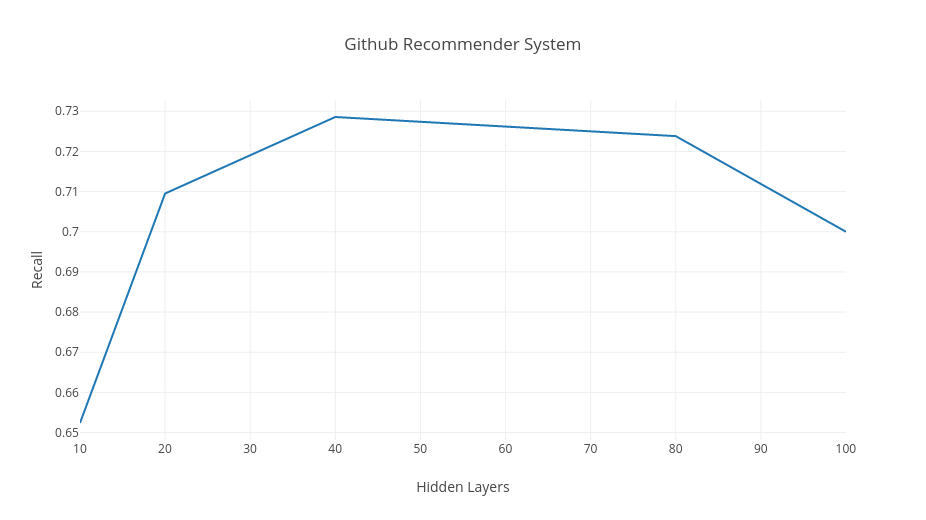
\includegraphics[width=\linewidth]{GRS.png}
    \caption{Recall vs Hidden Layers}
    \label{fig:1}
\end{figure*}
We used the user-based auto-encoder described in \cite{paper1} to train on our model. Firstly, each $r^{i}$ in the training dataset is partially observed, thus we only update the observed indices in $r^{i}$ while back-propagating. Secondly, we regularize the learned parameters to prevent over-fitting on the observed ratings. Formally, the objective function for the user-based model is as follows :\\\\
\resizebox{.5 \textwidth}{!} {$ \min_{\theta}\sum_{u} \|c_{u}\|_2 \|\left(p_{u} - h(r^{u};\theta)\right)\|_O^2 + \frac{\lambda}{2} \left(\sum_u \|W\|_F^2 + \sum_i \|V\|_F^2\right) $}
\begin{flushright}
-- (1)
\end{flushright}
\hspace{0.3in}where, $c_u = $ Confidence vector of user $u$, \\
      \hspace*{0.9in}$p_u = $ Preference vector of user $u$,\\
      \hspace*{0.9in}$||.||_O$ means, we consider the contributions\\ 
      \hspace*{1.2in}of only the observed ratings.\\
Once the model is trained then we can predict the preference matrix $R$ as follows:

    \[ R_{u,i} = \left(h(r^{u};\theta)\right)_{i} \]

Clearly, $R_{u,i} \in \{0, 1\}$, where, if $R_{u,i} = 1$, user $u$ would supposedly like the repository $i$.

\section{\textbf{Results}}
To test our model we do an 80:20 split of the data where $P_{u,i} = 1$ to get the test and train data respectively. We choose our test and train data this manner since, we are dealing with implicit ratings and hence do not have any negative feedback/dislike information.

To compare the prediction accuracy the standard metric of recall is used. Recall gives us the probability of a relevant repository being selected for recommendation. Mathematically,
    \[ Recall = \frac{t_p}{t_p + f_n} \]
\hspace{0.5in} where $t_p = $ number of true positives \\
\hspace*{0.85in} $f_p = $ number of false negatives

Many studies report results using one of the following metrics : MAE (Mean Absolute Error), RMSE (Root Mean Squared Error), NMAE (Normalized Mean Absolute Error) between the predicted and the ground truth values. But, using one of these metrics for testing the trained model does not make sense when one is dealing with implicit ratings because the predictions and the ground truth values belong to $\{0, 1\}$ which is a small set. Thus, the above mentioned metrics would also be small and would not give us the correct quantitative measure of the model's performance.

Precision is another information retrieval metric defined as follows,
    \[ Precision = \frac{t_p}{t_p + f_p} \]
\hspace{0.5in} where $t_p = $ number of true positives \\
\hspace*{0.85in} $f_n = $ number of false positives\\
Since, our test dataset does not contain any negative feedbacks thus, there are no false positives. This renders the use of this metric as meaningless. 
\subsection*{Hyper-parameter Tuning :}
\begin{itemize}
    \item We did a grid search on the following hyper-parameters:
        \begin{itemize}
            \item \textbf{Regularization Strength ($\lambda$)} over the set  $\{0.001, 0.01, 0.1\}$ and got best results for $\lambda_{best} = $ 0.01
            \item \textbf{Number of nodes in hidden layer ($k$)} over the set  $\{10, 20, 40, 80, 100\}$. Figure \ref{fig:1} shows that as we increase the hidden layer nodes from 40 to 80 nodes the model performs better, after 80 hidden layer nodes the recall value converges depicting \textbf{80} being \textbf{the best number of hidden layer nodes}.
        \end{itemize}
    \item \textbf{RMSProp optimizer} was used to minimize the loss function as described in equation (1).
    \item  We tested the trained model for both sigmoid and ReLU \textbf{hidden layer activation functions}. The model with hidden layer activation functions being the sigmoid function performed the best.
\end{itemize}

\section{\textbf{Future Work}}
\begin{itemize}
    \item Currently, we trained on our model on a 1000 x 1000 subset of the original 10K x 300K data collected. In the near future we plan on training on the entire dataset to get a better understanding of the trained model.
    \item  The auto-encoder model trained presently, has a single hidden layer. We could stack multiple hidden layers $i.e$ Stacked De-noising Auto-encoders(SdA) and report it's effect on the performance of the model.
    \item We can even try an item-based auto-encoder model and report it's effect on the model's performance.
\end{itemize}

\ifCLASSOPTIONcaptionsoff
  \newpage
\fi

% references section

% can use a bibliography generated by BibTeX as a .bbl file
% BibTeX documentation can be easily obtained at:
% http://www.ctan.org/tex-archive/biblio/bibtex/contrib/doc/
% The IEEEtran BibTeX style support page is at:
% http://www.michaelshell.org/tex/ieeetran/bibtex/
%\bibliographystyle{IEEEtran}
% argument is your BibTeX string definitions and bibliography database(s)
%\bibliography{IEEEabrv,../bib/paper}
%
% <OR> manually copy in the resultant .bbl file
% set second argument of \begin to the number of references
% (used to reserve space for the reference number labels box)
\begin{thebibliography}{1}

\bibitem{paper1}
\href{http://users.cecs.anu.edu.au/~akmenon/papers/autorec/autorec-paper.pdf}{\emph{Auto-Rec Paper}}\\
Suvash Sedhain†, Aditya Krishna Menon†, Scott Sanner†, Lexing Xie 

\bibitem{paper2}
\href{http://activisiongamescience.github.io/2016/01/11/Implicit-Recommender-Systems-Biased-Matrix-Factorization/#Implicit-Feedback}{\emph{Implicit Recommender System}}
\end{thebibliography}

% biography section
\end{document}


